%% Template.tex; Solar Physics
%% 
\documentclass[namedreferences]{solarphysics}
%
% spr-sola-addons available options:
%  natbib        -- For citations: redefine \cite commands (loads natbib.sty)
%  solaenum      -- makes enumerated list with italics-roman numerals and a single right-bracket\textbf{}
%  solaromanenum -- makes enumerated list with roman numerals and a single right-bracket
%  linksfromyear -- puts a link on a year citation (hyperref must be loaded)
%  optionalrh    -- for optional running title/author
%
\usepackage[optionalrh,solaromanenum]{spr-sola-addons} % For Solar Physics 
%\usepackage{epsfig}                     % For eps figures, old commands
\usepackage{graphicx}                    % For eps figures, newer & more powerfull
%\usepackage{courier}                    % Change the \texttt command to courier style
%\usepackage{amssymb}                    % useful mathematical symbols
\usepackage{color}                       % For color text: \color command
\usepackage{url}                         % For breaking URLs easily trough lines
\def\UrlFont{\sf}                        % define the fonts for the URLs


%% Local definitions
%% please place your own definitions here and don't use \def but
%% \newcommand{}{} or 
%% \renewcommand{}{} if it is already defined in LaTeX
\newcommand{\solphys}{{\it Solar Phys.}}
\newcommand{\aap}{    {\it Astron. Astrophys.}}
\newcommand{\aaps}{   {\it Astron. \& Astrophys. Supp.}}
\newcommand{\apj}{    {\it Astrophys. J.}}
\newcommand{\apjl}{    {\it Astrophys. J. Lett.}}
\newcommand{\apjs}{	{\it Astrophys. J. Supp. Ser.}}
\newcommand{\jgr}{    {\it J. Geophys. Res.}}
\newcommand{\aapr}{    {\it Astron. Astros Rev.}}
\newcommand{\grl}{    {\it Geophys. Res. Lett.}}
\newcommand{\lrsp}{    {\it Living Rev. Solar Phys.}}
\newcommand{\nat}{    {\it Nature}}
\newcommand{\asr}{{\it Adv. Space Res.}}
\newcommand{\ag}{	{\it Ann. Geophys.}}
\newcommand{\jastp}{	{\it J. Atmos. Solar-Terr. Phys.}}
\newcommand{\ssr}{	{\it Space Sci. Rev.}}
\newcommand{\ncomms}{	{\it Nat. Commun.}}
\newcommand{\natphys}{	{\it Nat. Phys.}}
\newcommand{\nasasp}{	{\it NASA SP-}}
\newcommand{\iausymp}{	{\it IAU Symp.}}


%%%%%%%%%%%%%%%%%%%%%%%%%%%%%%%%%%%%%%%%%%%%%%%%%%%%%%%%%%%%%%%%%%
\begin{document}

\begin{article}

\begin{opening}

\title{Off-pointed SWAP Obs.}

%%%%%%%%%%%%%%%%%%%%%%%%%%%%%%%%%%%%%%%%%%%%%%%%%%%
%% Authors Names
%
\author{J.\,P.~\surname{Byrne}$^{1}$\sep et al.
	%H.~\surname{Morgan}$^{2}$\sep
	%S.\,R.~\surname{Habbal}$^{1}$
       }

%%%%%%%%%%%%%%%%%%%%%%%%%%%%%%%%%%%%%%%%%%%%%%%%%%%
%% Runningheads
%
\runningauthor{Byrne et al.}
\runningtitle{Off-pointed SWAP Obs.}


%%%%%%%%%%%%%%%%%%%%%%%%%%%%%%%%%%%%%%%%%%%%%%%%%%%
%% Affilations 
%
  \institute{$^{1}$Institute for Astronomy, University of Hawaii, 2680 Woodlawn Drive, Honolulu, HI 96822, USA.
                     email: \url{jbyrne@ifa.hawaii.edu}\\ %email: \url{e.mail-b}
	%$^{2}$Sefydliad Mathemateg a Ffiseg, Prifysgol Aberystwyth, Ceredigion, Cymru, SY23 3BZ, UK.\\
%                     email: \url{e.mail-c} \\
             }


%%%%%%%%%%%%%%%%%%%%%%%%%%%%%%%%%%%%%%%%%%%%%%%%%%%
%%% Abstract 
\begin{abstract}

 
\end{abstract}



%%%%%%%%%%%%%%%%%%%%%%%%%%%%%%%%%%%%%%%%%%%%%%%%%%%
%% Keywords
%
\keywords{Coronal Mass Ejections, Low Coronal Signatures, Initiation and Propagation}


\end{opening}
%-------------------------------------------------

%%%%%%%%%%%%%%%%%%%%%%%%%%%%%%%%%%%%%%%%%%%%%%%%%%%
%% Sections
%

\section{Introduction}
\label{intro}



In this paper, relatively unique observations of a solar eruptive event are studied with a combination of multiple, overlapping EUV and white-light image data. In Section\,\ref{sect:techniques} we describe the observations and use of multiscale image processing methods. In Section\,\ref{sect:event} we describe the event, that occurred on 26~July~2013, and how the combination of observations and techniques can provide deeper insight into the initiation phase of CMEs. A discussion of the interpretation of this study is presented in Section\,\ref{sect:discussion}, and final conclusions in Section\,\ref{sect:conclusions}.

\section{Observations and Techniques}
\label{sect:techniques}


Data from solar-disk imagers may be combined with coronagraph observations, in order to connect CMEs to their source regions and study their initiation phase. The \emph{Sun Watcher using Active Pixel System Detector and Image Processing} (SWAP: \opencite{2013SoPh..286...43S}, \opencite{2013SoPh..286...67H}) on board the second \emph{Project for Onboard Autonomy} (PROBA2: \opencite{2013SoPh..286....5S}), has a spectral bandpass centered on 174\,{\AA}, with 3.2 arcsec pixels over a 54$\times$54 arcmin field-of-view, and a cadence of $\approx$\,2~minutes. It can be off-pointed to observe the extended EUV corona up to ?arcsecs, or ?R$_{\odot}$, which can overlap the white-light coronal observations to provide new insight to the initiation phase of CMEs.


\begin{figure}[ht]
\centering{\includegraphics[scale=0.6, trim=45 40 95 40, clip=true, width=\linewidth]{images/swap1830.pdf}}
\caption{SWAP images of a prominence eruption at 18:30\,UT on 26~July~2013 during a PROBA2 off-pointing campaign. The left image shows the results of a multiscale edge-detection algorithm, allowing a point-and-click characterization of the erupting structure. The right image shows the resulting ellipse fit overlaid on the original SWAP image (with a long-term background subtracted to highlight the faint EUV corona).}
\label{swap1830}
\end{figure}

\begin{figure}[ht]
\centering{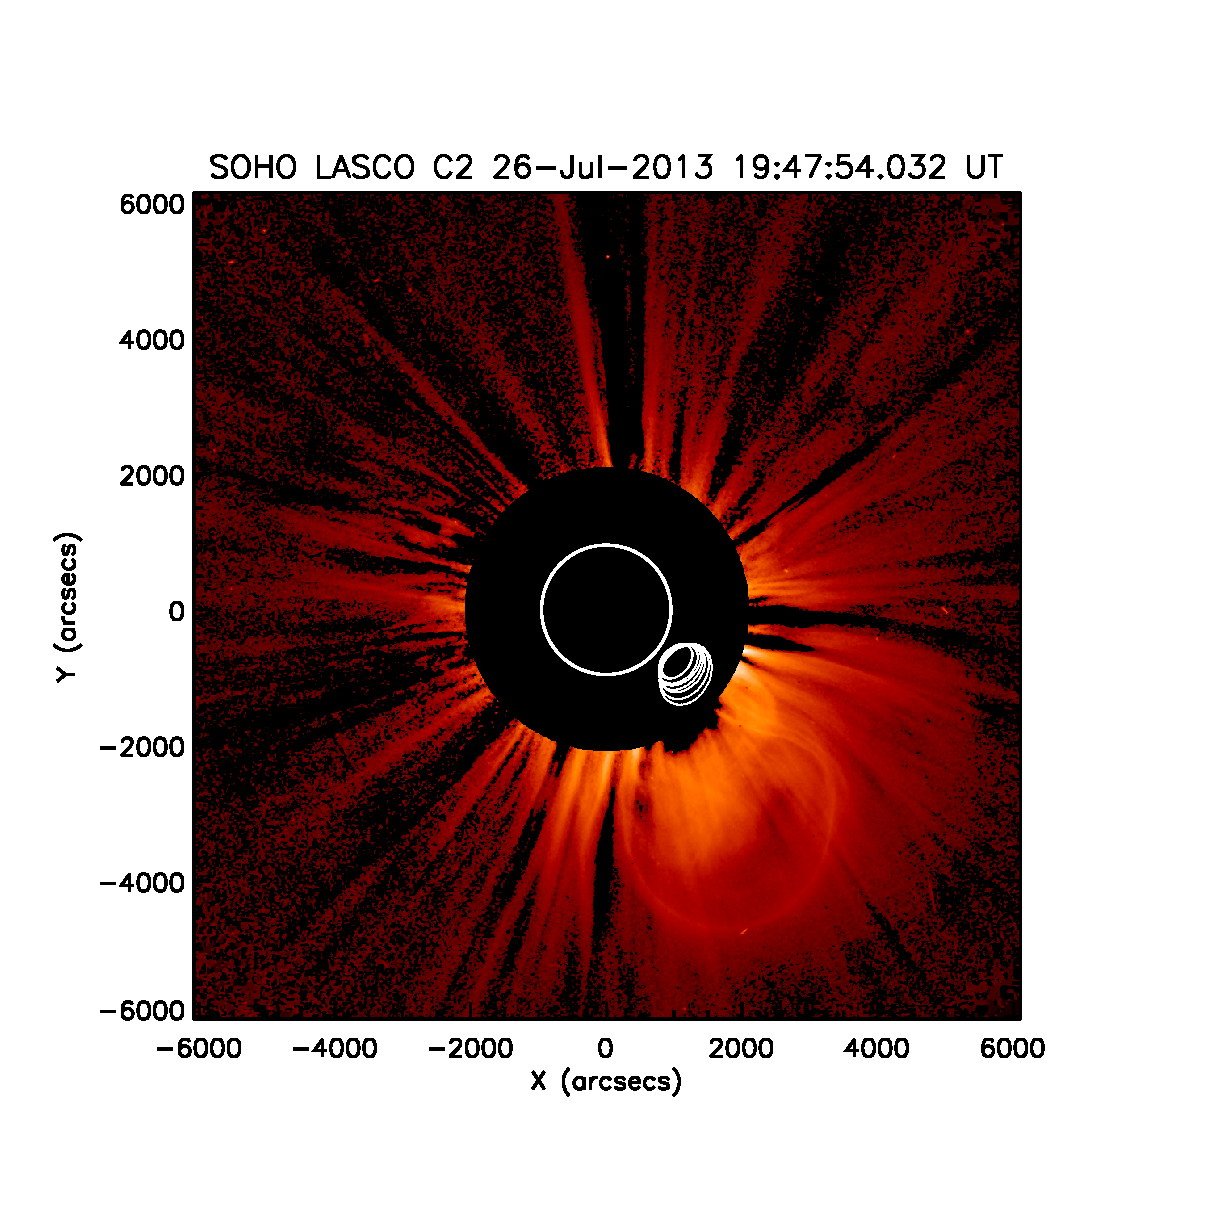
\includegraphics[trim=0 40 0 50, clip=true, width=\linewidth]{images/swap_ells_on_lasco_20130726_194754.eps}}
\caption{LASCO/C2 base-difference image of the CME at 19:47\,UT on 26~July~2013, with the ellipse characterizations from the SWAP observations of the associated prominence, overlaid on the plane-of-sky for comparison. It appears that the CME underwent a southward deflection or asymmetric expansion in its propagation.}
\label{swap_ells_on_lasco}
\end{figure}


 \emph{Extreme Ultraviolet Imager} (EUVI: \opencite{2004SPIE.5171..111W}) on board the \emph{Solar Terrestrial Relations Observatory} (STEREO: \opencite{2008SSRv..136....5K}), the \emph{Atmospheric Imaging Assembly} (AIA: \opencite{2012SoPh..275...17L}) on board the \emph{Solar Dynamics Observatory} (SDO: \opencite{2012SoPh..275....3P}); and the  \emph{Large Angle Spectrometric Coronagraph} (LASCO: \opencite{1995SoPh..162..357B}) on board the \emph{Solar and Heliospheric Observatory} (SOHO: \opencite{1995SoPh..162....1D}), and coronagraphs of the \emph{Sun-Earth Connection Coronal \& Heliospheric Imagers} (SECCHI: \opencite{}) on board STEREO. While there are difficulties in the interpretation of observations from the varying instruments (having different fields of view, image passbands, and cadences), the multiple viewpoints can complement each other to allow a determination of the true morphology of the system. 
 
Methods of multiscale image processing have been developed in recent years for use on solar image data to enhance the underlying structure \cite{2008ApJ...674.1201S,2008SoPh..248..457Y,2011AdSpR..47.2118G,2014SoPh..289.2945M}. The fundamental idea behind these methods is to highlight details apparent on different scales within the data. Therefore, multiscale techniques provide an ability to remove small-scale features in images, essentially suppressing the noise such that the structures of interest can be revealed in greater detail. By applying them to coronagraph images, the morphology of CMEs as they propagate through the corona in a sequence of observations can be determined with better accuracy than previously possible, and can allow a characterization of the erupting structure to determine various properties in their evolution (\opencite{2009A&A...495..325B}, \citeyear{2010NatCo...1E..74B}, \citeyear{2012ApJ...752..145B}). 

Here, multiscale methods are used on observations from the disk imaging instruments of SDO/AIA, STEREO/SECCHI-EUVI, and SWAP EUV imager, to provide insight into the low-coronal morphology of erupting structures that form CMEs. Details on the fundamental techniques are outlined in \inlinecite{2008SoPh..248..457Y} wherein the magnitude of the multiscale gradient is used to show the relative strength of the detected edges in the image structure at a particular scale of the multiscale decomposition (\emph{i.e.}, the strongest edges appear brightest). To further increase the signal-to-noise ratio of the edge detections, the magnitude information from the scales most relevant to the coronal structures of interest may be multiplied together, neglecting the largest scales that smooth out the coronal signal, and the smallest scales that reveal the finer structure and noise (see \opencite{2012ApJ...752..145B}, for details). Thus the magnitude of the multiscale gradient across the dominant edges of coronal loops and CMEs is further enhanced for subsequent characterization of their morphology. 

\inlinecite{2014arXiv1406.4919B} show the effectiveness of the multiscale techniques for detecting the structure of an ejection in SWAP images. These multiscale methods are applied to the SWAP data here, for this event seen during the off-pointing campaign on 26~July~2013, in order to highlight the structures in the image and perform a point-and-click characterization of the erupting prominence. This allows, for example, an ellipse fit to the outward propagating fronts, to obtain kinematical and morphological information as described in \inlinecite{2009A&A...495..325B}. Figure\,\ref{swap1830} shows two images of the SWAP observations of the erupting prominence at 18:30\,UT on 26\,July\,2013:



\section{Solar Eruptive Event}
\label{sect:event}




\section{Discussion}
\label{sect:discussion}



\section{Conclusions}
\label{sect:conclusions}




%%%%%%%%%%%%%%%%%%%%%%%%%%%%%%%%%%%%%%%%%%%%%%%%%%%%%%%%%%%%%%%%%%%%%%%%%%%
%% Acknowledgements
%
 \begin{acks}
 
This work is supported by SHINE grant 0962716 and NASA grants NNX08AJ07G and NNX13AG11G to the Institute for Astronomy.
SWAP is a project of the Centre Spatial de Li\'ege and the Royal Observatory of Belgium funded by the Belgian Federal Science Policy Office (BELSPO).
The SOHO/LASCO data used here are produced by a consortium of the Naval Research Laboratory (USA), Max-Planck-Institut fuer Aeronomie (Germany), Laboratoire d'Astronomie (France), and the University of Birmingham (UK). SOHO is a project of international cooperation between ESA and NASA.
SDO data supplied is a courtesy of the NASA/SDO consortia. JPB is grateful to have been a PROBA2 Guest Investigator.
% The authors thank the anonymous referee for their helpful comments.

 \end{acks}


%%% %%%%%%%%%%%%%%%%%%%%%%%%%%%%%%%%%%%%%%%%%%%%%%%%%%%%%%%%%%%
%% Bibliography
%
% Using BibTeX
%
 \bibliographystyle{spr-mp-sola.bst}
% %\bibliographystyle{spr-mp-sola-cnd} %% Alternative style: no title, no concluding page
 \bibliography{references.bib}  
%
% Without BibTeX 
% \begin{thebibliography}{}
% \bibitem[\protect\citeauthoryear{Author}{Year}]{key}
%   <bibliographical entry>
%
% \bibitem[\protect\citeauthoryear{}{}]{}
%   
%  
% \end{thebibliography}

\end{article} 
\end{document}
